%
% 2-tensor.tex
%
% (c) 2023 Prof Dr Andreas Müller
%
\section{Das Kronecker-Produkt
\label{buch:diskret:section:tensor}}
Im vorangegangenen Abschnitt wurde gezeigt, dass sich kompliziertere
Gruppen aus zyklischen Gruppen mit Primzahl-Ordnung als Produkt
zusammensetzen lassen.
In diesem Abschnitt soll daher untersucht werden, wie Funktionen auf
einem Produkt $X\times Y$ aus Funktionen auf den Faktoren $X$ und $Y$
zusammengesetzt werden können.
Dabei ergibt sich das sogenannte Tensor-Produkt.

%
%
%
\subsection{Kartesisches Produkt als Definitionsbereich
\label{buch:diskret:section:}}
Seien $X$ und $Y$ endliche Mengen und seien $f\in\mathbb{C}^X$ und 
$g=\mathbb{C}^Y$ Funktionen auf den Mengen $X$ und $Y$.
Das Produkt der Funktionen $f$ und $g$ ist die Funktion
\[
h
\colon
X\times Y \to \mathbb{C}
:
(x,y)
\mapsto
h(x,y) = f(x)g(y).
\]
Sie wird im Folgenden auch mit $f\otimes g$ bezeichnet und das
{\em Tensor-Produkt} von $f$ und $g$ genannt.

Dies Produkt hat die Eigenschaften
\begin{align*}
(f_1+f_2)\otimes g &= f_1\otimes g + f_2\otimes g
&
f\otimes(g_1+g_2) &= g_1\otimes f + g_2\otimes f
\\
(\lambda f)\otimes g &= \lambda (f\otimes g)
&
f\otimes(\lambda g) &= \lambda (f\otimes g),
\end{align*}
es ist also linear in beiden Faktoren.
Die beiden unteren Identitäten besagen aber auch, dass
$\lambda f\otimes g = f\otimes \lambda g$, skalare Faktoren
lassen sich also beliebig zwischen den Faktoren des
Tensorproduktes hin und her schieben.

%
% Basis
%
\subsubsection{Basen}
Die Standardbasis der Vektorräume $\mathbb{C}^X$ und $\mathbb{C}^Y$
der Funktionen auf $X$ bzw.~$Y$
besteht aus den Funktionen
\[
e_x(\xi)
=
\begin{cases}
1&\qquad x=\xi\\
0&\qquad\text{sonst}
\end{cases}
\qquad\text{bzw.}\qquad
e_y(\eta)
=
\begin{cases}
1&\qquad y=\eta\\
0&\qquad\text{sonst.}
\end{cases}
\]
Die Standardbasis von $\mathbb{C}^{X\times Y}$ besteht aus den Funktionen
\[
e_{x,y}(\xi,\eta)
=
\begin{cases}
1&\qquad\text{$x=\xi$ und $y=\eta$}\\
0&\qquad\text{sonst}
\end{cases}
\]
Diese lassen sich auch als Tensor-Produkte schreiben, nämlich
$e_{x,y} = e_x\otimes e_y$.

Die Funktionen $f\colon X\to \mathbb{C}$ und $g\colon Y\to\mathbb{C}$
lässt sich in den Standardbasen als Linearkombinationen
\[
f = \sum_{x\in X} f(x)e_x
\qquad\text{und}\qquad
g = \sum_{y\in Y} g(y)e_y
\]
schreiben.

Da das Tensorprodukt linear in beiden Faktoren ist, ist das Tensorprodukt
von $f$ und $g$ daher
\[
f\otimes g
=
\sum_{x\in X}\sum_{y\in Y}
f(x)g(y) e_x\otimes e_y
=
\sum_{(x,y)\in X\times Y}
(f\otimes g)(x,y) e_x\otimes e_y
\]

%
% Das Tensorprodukt
%
\subsubsection{Das Tensorprodukt $U\otimes V$}
Die Überlegungen des vorangegangenen Abschnitts liefert nicht nur
eine Beschreibung des Vektorraums $\mathbb{C}^{X\times Y}$.
Sie kann nämlich auf zwei beliebige Vektorräume
$U$ und $V$ verallgemeinert werden.
Dazu seien $\mathcal{B}=\{u_1,\dots,u_n\}$ und $\mathcal{C}=\{v_1,\dots,v_m\}$
Basen der Vektorräume.
Jeder Vektor in $U$ kann als Linearkombination von Vektoren aus
$\mathcal{B}$ geschrieben werden, ebenso kann jeder Vektor von $V$
als Linearkombination von Vektoren in $\mathcal{C}$ geschrieben werden.
Die Basisvektoren übernehmen dabei die Rollen der Funktionen
$e_x\in \mathbb{C}^X$ und $e_y\in\mathbb{C}^Y$.
Wir definieren daher einen neuen Vektorraum $U\otimes V$ mit
der Basis
\[
\mathcal{B}\otimes\mathcal{C}
=
\{
u_i\otimes v_j
\mid
i=1,\dots,n\text{ und }j=1,\dots,m
\}.
\]
Der Vektorraum $U\otimes V$ besteht also aus Linearkombinationen
\[
\sum_{i=1}^n \sum{j=1}^m
a_{ij} u_i\otimes v_j
\]
von Tensorprodukten $u_i\otimes v_j$.

Der Vektorraum $U\otimes V$ ist kleiner als das kartesische Produkt
$U\times V$, da die Vektoren
\[
(\lambda u_i)\otimes v_j
=
u_i\otimes (\lambda v_j)
=
\lambda (u_i\otimes v_j)
\]
in $U\otimes V$ alle als gleich betrachtet werden, während die
Paare $(\lambda u_i,v_j)$ und $(u_i,\lambda v_j)$ verschieden sind.

Der Vektorraum $U\otimes V$ berücksichtigt, dass eine bilineare Abbildung
ebenfalls die Eigenschaft hat, dass ein skalarer Faktor vom einen
Argument auf das andere geschoben werden kann:
\[
f(\lambda x,y) = f(x,\lambda y) = \lambda f(x,y)
\]
für eine auf $U\times V$ definierte lineare Abbildung $f$.
Daher hat der Vektorraum $U\otimes V$ hat die folgende universelle
Eigenschaft.
Ist $f\colon U\times V\to W$ eine {\em bilineare} Abbildung, dann
gibt es auch eine eindeutig bestimmte {\em lineare} Abbildung
$g\colon U\otimes V\to W$ derart, dass
\[
f(u,v)
=
g(u\otimes v).
\]
Da die Vektoren $u_i\otimes v_j$ eine Basis von $U\otimes V$ bilden,
ist $g$ als lineare Abbildung durch $g(u_i\otimes v_j) = f(u_i,v_j)$
vollständig definiert.

Das Tensorprodukt von Funktionen im vorangegangenen Abschnitt besteht
aus Elementen des Tensorprodukts der Vektorräume
$\mathbb{C}^X\otimes \mathbb{C}^Y = \mathbb{C}^{X\times Y}$.

%
% Lineare Abbildungen
%
\subsection{Lineare Abbildungen
\label{buch:diskret:tensor:subsection:linabb}}
Eine lineare Abbildung $\mathbb{C}^X\to \mathbb{C}^X$ wird durch eine
Matrix $A$ mit Einträgen $a_{xx'}$ beschrieben.
Die Bildfunktion $Af$ ist definiert durch
\[
(Af)(x) = \sum_{x'\in X}a_{xx'}f(x')
\qquad\Rightarrow\qquad
Af = \sum_{x,x'\in X} a_{xx'}f(x') e_x
\]
Entsprechend wird eine lineare Abbildung $\mathbb{C}^Y\to\mathbb{C}^Y$
durch eine Matrix $B$ mit den Einträgen $b_{yy'}$ beschrieben.

Aus den beiden Abbildungen lässt sich jetzt eine Abbildung 
$\mathbb{C}^{X\times Y} \to \mathbb{C}^{X\times Y}$
konstruieren, sie bildet die Funktion $f\otimes g$ auf die
Funktion
\[
(Af\otimes Bg)(x,y)
=
(Af)(x)\cdot (Bg)(y)
=
\sum_{(x',y')\in X\times Y}
a_{xx'}f(x') b_{yy'}g(y')
\]
oder
\[
(A\otimes B)
(f\otimes g)
=
Af\otimes Bg
=
\sum_{(x,y)\in X\times Y}
\biggl(
\sum_{(x',y')\in X\times Y}
\underbrace{a_{xx'}b_{yy'}}_{c_{\displaystyle (x,y),(x',y')}}
f(x')g(y')
\biggr)
e_x\otimes e_y.
\]
Die lineare Abbildung $A\otimes B$ wird in der Basis $e_x\otimes e_y$
durch die Koeffizienten
\[
c_{(x,y),(x',y')}
=
a_{xx'}b_{yy'}
\]
beschrieben werden.

%
% Matrizen
%
\subsection{Matrizen
\label{buch:diskret:tensor:subsection:matrizen}}
Um die Matrizen $A$, $B$ und $C$ in der üblichen Art als rechteckiges
Zahlenschema darzustellen, muss eine Reihenfolge der Elemente von $X$,
$Y$ und $X\times Y$ gewählt werden.
Dazu schreiben wir $X=\{1,\dots,n\}$ und $Y=\{1,\dots,m\}$.
Die linearen Abbildungen $A$ und $B$ haben dann die Matrizen
\[
A
=
\begin{pmatrix}
a_{11}&a_{12}&\dots &a_{1n}\\
a_{21}&a_{22}&\dots &a_{2n}\\
\vdots&\vdots&\ddots&\vdots\\
a_{n1}&a_{n2}&\dots &a_{nn}
\end{pmatrix}
\qquad\text{und}\qquad
B
=
\begin{pmatrix}
b_{11}&b_{12}&\dots &b_{1m}\\
b_{21}&b_{22}&\dots &b_{2m}\\
\vdots&\vdots&\ddots&\vdots\\
b_{m1}&b_{m2}&\dots &b_{mm}
\end{pmatrix}.
\]
Um auch die Abbildung $C$ als Matrix zu schreiben, muss das kartesische
Produkt $X\times Y$ angeordnet werden.
Eine natürlich Anordnung ist die lexikographische:
\[
(1,1), (1,2),\dots,(1,m),(2,1),(2,2),\dots,(2,m),\dots,(n,1),(n,2),\dots,(n,m).
\]
In dieser Reihenfolge können die Koeffizienten von $C=A\otimes B$ als
\bgroup
\def\w{1.2}%
\def\h{0.8}%
\def\punkt#1#2{({(#2)*\w},{-(#1)*\h})}%
\def\Hdots#1#2{
	\foreach \y in {-0.2,0,0.2}{
		\fill \punkt{#1}{#2+(\y)/\w} circle[radius=0.02];
	}
}%
\def\Vdots#1#2{
	\foreach \x in {-0.2,0,0.2}{
		\fill \punkt{#1+(\x)/\h}{#2} circle[radius=0.02];
	}
}%
\def\Ddots#1#2{
	\foreach \u in {-0.2,0,0.2}{
		\fill \punkt{#1+(\u)/\h}{#2+(\u)/\w} circle[radius=0.02];
	}
}%
\begin{align}
C
=
A\otimes B
&=
\left(%
\raisebox{-3.3cm}{%
\def\block#1#2{
\node at \punkt{0}{0} {$a_{#1#2}b_{11}$};
\Hdots{0}{0.75}
\node at \punkt{0}{1.5} {$a_{#1#2}b_{1m}$};
\Vdots{0.75}{0}
\Ddots{0.75}{0.75}
\Vdots{0.75}{1.5}
\node at \punkt{1.5}{0} {$a_{#1#2}b_{m1}$};
\Hdots{1.5}{0.75}
\node at \punkt{1.5}{1.5} {$a_{#1#2}b_{mm}$};
}%
\begin{tikzpicture}[>=latex,thick]
\begin{scope}
	\begin{scope}
		\block{1}{1}
	\end{scope}
	\begin{scope}[xshift=3.0cm]
		\block{1}{2}
	\end{scope}
	\Hdots{0.75}{5}
	\begin{scope}[xshift=7.2cm]
		\block{1}{n}
	\end{scope}
\end{scope}
\begin{scope}[yshift=-2cm]
	\begin{scope}
		\block{2}{1}
	\end{scope}
	\begin{scope}[xshift=3.0cm]
		\block{2}{2}
	\end{scope}
	\Hdots{0.75}{5}
	\begin{scope}[xshift=7.2cm]
		\block{2}{n}
	\end{scope}
\end{scope}
\begin{scope}[yshift=-4.0cm]
	\Vdots{0}{0.75}
	\Vdots{0}{3.25}
	\Ddots{0}{5}
	\Vdots{0}{6.75}
\end{scope}
\begin{scope}[yshift=-4.8cm]
	\begin{scope}
		\block{n}{1}
	\end{scope}
	\begin{scope}[xshift=3.0cm]
		\block{n}{2}
	\end{scope}
	\Hdots{0.75}{5}
	\begin{scope}[xshift=7.2cm]
		\block{n}{n}
	\end{scope}
\end{scope}
\draw[color=gray] \punkt{-0.5}{2} -- \punkt{8}{2};
\draw[color=gray] \punkt{-0.5}{4.5} -- \punkt{8}{4.5};
\draw[color=gray] \punkt{-0.5}{5.5} -- \punkt{8}{5.5};
\draw[color=gray] \punkt{2}{-0.5} -- \punkt{2}{8};
\draw[color=gray] \punkt{4.5}{-0.5} -- \punkt{4.5}{8};
\draw[color=gray] \punkt{5.5}{-0.5} -- \punkt{5.5}{8};
\end{tikzpicture}}
\right)
\label{buch:diskret:tensor:eqn:kronecker1}
\intertext{
dargestellt werden.
Sie kann auch als Blockmatrix mit Blöcken der der Form $a_{ik}B$
geschrieben werden:}
A\otimes B
&=
\def\h{1.3}
\def\w{1.3}
\left(%
\raisebox{-2.2cm}{\begin{tikzpicture}[>=latex,thick]
\node at \punkt{0}{0} {$a_{11}B$};
\node at \punkt{0}{1} {$a_{12}B$};
\Hdots{0}{1.8}
\node at \punkt{0}{2.6} {$a_{1n}B$};
\node at \punkt{1}{0} {$a_{21}B$};
\node at \punkt{1}{1} {$a_{22}B$};
\Hdots{1}{1.8}
\node at \punkt{1}{2.6} {$a_{2n}B$};
\Vdots{1.8}{0}
\Vdots{1.8}{1}
\Ddots{1.8}{1.8}
\Vdots{1.8}{2.6}
\node at \punkt{2.6}{0} {$a_{n1}B$};
\node at \punkt{2.6}{1} {$a_{n2}B$};
\Hdots{2.6}{1.8}
\node at \punkt{2.6}{2.6} {$a_{nn}B$};
\draw[color=gray] \punkt{0.5}{-0.5} -- \punkt{0.5}{3.1};
\draw[color=gray] \punkt{1.5}{-0.5} -- \punkt{1.5}{3.1};
\draw[color=gray] \punkt{2.1}{-0.5} -- \punkt{2.1}{3.1};
\draw[color=gray] \punkt{-0.5}{0.5} -- \punkt{3.1}{0.5};
\draw[color=gray] \punkt{-0.5}{1.5} -- \punkt{3.1}{1.5};
\draw[color=gray] \punkt{-0.5}{2.1} -- \punkt{3.1}{2.1};
\end{tikzpicture}}%
\right).
\label{buch:diskret:tensor:eqn:kronecker2}
\end{align}
\egroup
Die Matrix $A\times B$ gemäss
\eqref{buch:diskret:tensor:eqn:kronecker1}
oder
\eqref{buch:diskret:tensor:eqn:kronecker2}
heisst das {\em Kronecker-Produkt} der Matrizen $A$ und $B$.
\index{Kronecker-Produkt}%

Die Definition des Kronecker-Produktes von Matrizen funktioniert
natürlich auch für rechteckige Matrizen.
Ist $A$ eine $n\times r$-Matrix und $B$ eine $m\times s$-Matrix,
dann ist $A\otimes B$ eine $nm\times rs$-Matrix, die sich aus
$m\times s$-Blöcken der Form $a_{ik}B$, die in einem $n\times r$-Gitter
angeordnet sind.

%
% Kroneckerprodukt mit einer Einheitsmatrix
%
\subsection{Kroneckerprodukt mit einer Einheitsmatrix}
Besonders übersichtlich wird das Kronecker-Produkt, wenn einer
der Faktoren eine Einheitsmatrix ist.
Ist $B=I_m$ eine $m$-dimensionale Einheitsmatrix, dann ist
\begin{equation}
A\otimes B
=
A\otimes I_m
=
\left(
\raisebox{-1.65cm}{%
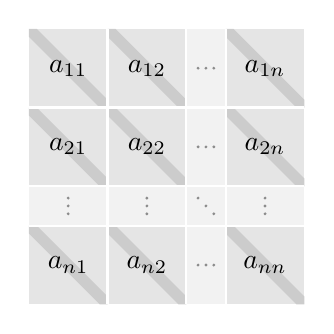
\begin{tikzpicture}[>=latex,thick]
\def\diagonale#1#2{
	\fill[color=gray!40] (#1,#2) -- ++(0.1,0) -- ++(0.9,-0.9) -- ++(0,-0.1) -- ++(-0.1,0) -- ++(-0.9,0.9) -- cycle;
}
\def\Vdots#1#2{
	\foreach \y in {-1,0,1}{
		\fill[color=gray!90] (#1,{#2+(\y)*0.1}) circle[radius=0.02];
	}
}
\def\Hdots#1#2{
	\foreach \x in {-1,0,1}{
		\fill[color=gray!90] ({#1+(\x)*0.1},#2) circle[radius=0.02];
	}
}
\def\Ddots#1#2{
	\foreach \x in {-1,0,1}{
		\fill[color=gray!90] ({#1+(\x)*0.1},{#2-(\x)*0.1}) circle[radius=0.02];
	}
}
\fill[color=gray!20] (0,0) rectangle (3.5,-3.5);
\fill[color=gray!10] (0,-2) rectangle (3.5,-2.5);
\fill[color=gray!10] (2,0) rectangle (2.5,-3.5);
\diagonale{0}{0}
\diagonale{1}{0}
\Hdots{2.25}{-0.5}
\diagonale{2.5}{0}
%
\diagonale{0}{-1}
\diagonale{1}{-1}
\Hdots{2.25}{-1.5}
\diagonale{2.5}{-1}
%
\Vdots{0.5}{-2.25}
\Vdots{1.5}{-2.25}
\Ddots{2.25}{-2.25}
\Vdots{3}{-2.25}
%
\diagonale{0}{-2.5}
\diagonale{1}{-2.5}
\Hdots{2.25}{-3}
\diagonale{2.5}{-2.5}
\foreach \y in {-1,-2,-2.5}{
	\draw[color=white] (0,\y) -- (3.5,\y);
}
\foreach \x in {1,2,2.5}{
	\draw[color=white] (\x,0) -- (\x,-3.5);
}
\node at (0.5,-0.5) {$a_{11}$};
\node at (1.5,-0.5) {$a_{12}$};
\node at (3.0,-0.5) {$a_{1n}$};
\node at (0.5,-1.5) {$a_{21}$};
\node at (1.5,-1.5) {$a_{22}$};
\node at (3.0,-1.5) {$a_{2n}$};
\node at (0.5,-3.0) {$a_{n1}$};
\node at (1.5,-3.0) {$a_{n2}$};
\node at (3.0,-3.0) {$a_{nn}$};
\end{tikzpicture}}
\right)
\label{buch:diskret:tensor:eqn:AIm}
\end{equation}
$A\otimes B=A\otimes I_m$ eine Matrix aus $m\times m$ grossen
Blöcken, die jeweils diagonal sind und auf der Diagonalen
die $n\times n$ Werte $a_{ik}$ haben.

Ist hingegen $A=I_n$ eine $n$-dimensionale Diagonalmatrix, dann ist
\begin{equation}
A\otimes B
=
I_n\otimes B
=
\left(\raisebox{-1.65cm}{%
\def\Ddots#1#2{
	\foreach \x in {-1,0,1}{
		\fill ({#1+(\x)*0.1},{#2-(\x)*0.1}) circle[radius=0.02];
	}
}%
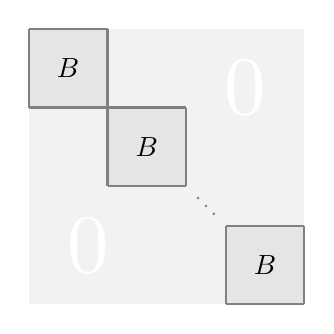
\begin{tikzpicture}[>=latex,thick]
\fill[color=gray!10] (0,0) rectangle (3.5,-3.5);
\fill[color=gray!20] (0,0) rectangle (1,-1);
\fill[color=gray!20] (1,-1) rectangle (2,-2);
\fill[color=gray!20] (2.5,-2.5) rectangle (3.5,-3.5);
\node at (0.5,-0.5) {$B$};
\node at (1.5,-1.5) {$B$};
\node at (3.0,-3.0) {$B$};
\draw[color=gray] (0,0) -- (1,0);
\draw[color=gray] (0,-1) -- (2,-1);
\draw[color=gray] (1,-2) -- (2,-2);
\draw[color=gray] (2.5,-2.5) -- (3.5,-2.5);
\draw[color=gray] (2.5,-3.5) -- (3.5,-3.5);
\draw[color=gray] (0,0) -- (0,-1);
\draw[color=gray] (1,0) -- (1,-2);
\draw[color=gray] (2,-1) -- (2,-2.0);
\draw[color=gray] (2.5,-2.5) -- (2.5,-3.5);
\draw[color=gray] (3.5,-2.5) -- (3.5,-3.5);
\Ddots{2.25}{-2.25}
\node[color=white,scale=3] at (2.75,-0.75) {$0$};
\node[color=white,scale=3] at (0.75,-2.75) {$0$};
\end{tikzpicture}}
\right)
\label{buch:diskret:tensor:eqn:InB}
\end{equation}
eine Matrix von diagonalen $m\times m$-Blöcken,
die alle nur die Matrix $B$ enthalten.

Aus den beiden oben gefundenen Regeln lässt sich jetzt sofort
ableiten, dass das Kronecker-Produkt zweier Einheitsmatrizen
$I_p$ und $I_q$ die Einheitsmatrix
\[
I_p\otimes I_q = I_{pq}
\]
ist.

%
% Assoziativität
%
\subsubsection{Assoziativität}
Das Kronecker-Produkt ist assoziativ, wie man aus der Konstruktion
unmittelbar ablesen kann.
Das Produkt
\[
A\otimes B\otimes C
=
\left(\raisebox{-2.5cm}{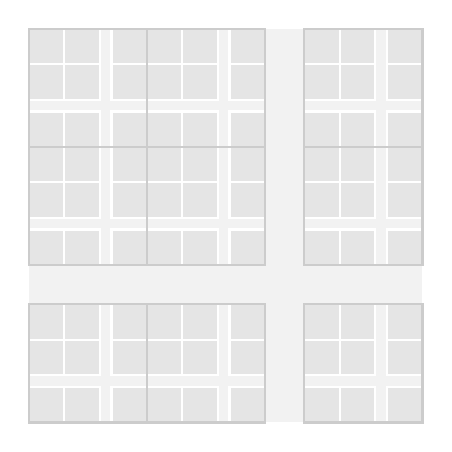
\begin{tikzpicture}[>=latex,thick,scale=0.5]

\fill[color=gray!10] (0,0) rectangle (10,-10);
\fill[color=gray!20] (0,0) rectangle (1.8,-1.8);
\fill[color=gray!20] (2.1,0) rectangle (4.8,-1.8);
\fill[color=gray!20] (5.1,0) rectangle (6,-1.8);
\fill[color=gray!20] (7,0) rectangle (8.8,-1.8);
\fill[color=gray!20] (9.1,0) rectangle (10,-1.8);

\fill[color=gray!20] (0,-2.1) rectangle (1.8,-4.8);
\fill[color=gray!20] (2.1,-2.1) rectangle (4.8,-4.8);
\fill[color=gray!20] (5.1,-2.1) rectangle (6,-4.8);
\fill[color=gray!20] (7,-2.1) rectangle (8.8,-4.8);
\fill[color=gray!20] (9.1,-2.1) rectangle (10,-4.8);

\fill[color=gray!20] (0,-5.1) rectangle (1.8,-6);
\fill[color=gray!20] (2.1,-5.1) rectangle (4.8,-6);
\fill[color=gray!20] (5.1,-5.1) rectangle (6,-6);
\fill[color=gray!20] (7,-5.1) rectangle (8.8,-6);
\fill[color=gray!20] (9.1,-5.1) rectangle (10,-6);

\fill[color=gray!20] (0,-7) rectangle (1.8,-8.8);
\fill[color=gray!20] (2.1,-7) rectangle (4.8,-8.8);
\fill[color=gray!20] (5.1,-7) rectangle (6,-8.8);
\fill[color=gray!20] (7,-7) rectangle (8.8,-8.8);
\fill[color=gray!20] (9.1,-7) rectangle (10,-8.8);

\fill[color=gray!20] (0,-9.1) rectangle (1.8,-10);
\fill[color=gray!20] (2.1,-9.1) rectangle (4.8,-10);
\fill[color=gray!20] (5.1,-9.1) rectangle (6,-10);
\fill[color=gray!20] (7,-9.1) rectangle (8.8,-10);
\fill[color=gray!20] (9.1,-9.1) rectangle (10,-10);

\def\rklein#1#2{
	\draw[color=white] ({#1},{#2}) rectangle ({(#1)+0.9},{(#2)-0.9});
}

\def\rgross#1#2{
	\foreach \ox in {0,0.9,2.1}{
		\foreach \oy in {0,-0.9,-2.1}{
			\rklein{#1+\ox}{#2+\oy}
		}
	}
	\draw[color=gray!40] ({#1},{#2}) rectangle ({(#1)+3},{(#2)-3});
}

\foreach \x in {0,3,7}{
	\foreach \y in {0,-3,-7}{
		\rgross{\x}{\y}
	}
}

\end{tikzpicture}}\right)
\]
besteht aus Blöcken, die Kopien von $C$ sind, multipliziert mit
den Matrixelementen von $A\otimes B$.

Wegen $I_p\otimes I_q=I_{pq}$ sind die Produkte mit Einheitsmatrizen
wieder besonders übersichtlich.
Es gilt
\begin{equation}
(A\otimes I_p)\otimes I_q
=
A\otimes I_{pq}
\qquad\text{und}\qquad
I_p\otimes (I_q\otimes B)
=
I_{pq}\otimes B.
\label{buch:diskret:tensor:eqn:assozi}
\end{equation}

%
%  Zusammensetzung
%
\subsection{Zusammensetzung
\label{buch:diskret:tensor:subsection:zusammensetzung}}
Aus der Definition des Tensorproduktes von linearen Abbildungen folgt
auch eine Regel, wie die Tensorproduktabbildungen zusammengesetzt
werden müssen.
Seien $A_1$ und $A_2$ $n\times n$-Matrizen mit Matrixelementen
$a_{xx'}^{(k)}$, $x,x'\in X$ und $k=1,2$.
Ausserdem seien $B_k$ $m\times m$-Matrizen mit Matrixelementen
$b_{yy'}^{(k)}$ mit $y,y'\in Y$ und $k=1,2$.
Das Tensorprodukt $A_k\otimes B_k$ hat die Matrixelemente
\[
c_{(x,y),(x',y')}^{(k)}
=
a_{xx'}^{(k)}
b_{yy'}^{(k)}.
\]
Die Zusammensetzung $(A_1\otimes B_1)(A_2\otimes B_2)$ hat die
Matrixelemente
\begin{align*}
c_{(x,y),(x',y')}
&=
\sum_{(x'',y'')\in X\times Y}
c^{(1)}_{(x,y),(x'',y'')}
c^{(2)}_{(x'',y''),(x',y')}
\\
&=
\sum_{(x'',y'')\in X\times Y}
a^{(1)}_{xx''} a^{(2)}_{x''x'}
b^{(1)}_{yy''} b^{(2)}_{y''y'}
\\
&=
\biggl(
\sum_{x''\in X}
a^{(1)}_{xx''} a^{(2)}_{x''x'}
\biggr)
\biggl(
\sum_{y''\in Y}
b^{(1)}_{yy''} b^{(2)}_{y''y'},
\biggr)
\end{align*}
dies sind die Matrixelemente von $A_1A_2 \otimes B_1B_2$.

\begin{satz}
Seien
$A_k\in M_{n\times n}(\Bbbk)$ und $B_k\in M_{m\times m}(\Bbbk)$
für $k=1,2$.
Dann gilt
\[
(A_1\otimes B_1)(A_2\otimes B_2)
=
(A_1A_2)\otimes (B_1B_2).
\]
Die Matrix $I_n\otimes I_m$ ist die Einheitsmatrix.
Sind $A\in M_{n\times n}(\Bbbk)$ und $B\in M_{m\times m}(\Bbbk)$ 
invertierbar, dann gilt
\[
(A\otimes B)^{-1}
=
A^{-1}\otimes B^{-1}.
\]
\end{satz}

%
% Determinante
%
\subsection{Determinante von $A\otimes B$
\label{buch:diskret:tensor:subsection:determinante}}
Aus der Zusammensetzungsregel für Tensorproduktabbildungen folgt
\[
A\otimes B
=
(A\otimes I_m)(I_n\otimes B).
\]
Somit kann die Determinante von $A\otimes B$ mit Hilfe der
Produktregel
\[
\det (A\otimes B)
=
\det(A\otimes I_m)
\det(I_n\otimes B)
\]
berechnet werden.

\begin{satz}
\label{buch:diskret:tensor:satz:deteinheit}
Für $A\in M_{n\times n}(\Bbbk)$ und $B\in M_{m\times m}(\Bbbk)$ ist
\[
\det (A\otimes I_m) = \det(A)^m
\qquad\text{und}\qquad
\det (I_n\otimes B) = \det(B)^n.
\]
\end{satz}

\begin{proof}[Beweis]
Die Matrix $I_n\otimes B$ ist eine Blockmatrix mit Blöcken $B$ auf
der Diagonalen.
Die Determinante einer solchen Blockmatrix ist das Produkt der
Determinanten der diagonalen Blöcke, also
\[
\det(I_n\otimes B) = \det(B)^n.
\]
Die Matrix $A\otimes I_m$ besteht aus $m$ Kopien von $A$, die aber
nicht wie im Falle von $I_n\otimes B$ in der Matrix nebeneinander
stehen.
Stattdessen sind die Zeilen und Spalten umgegeordnet, zuerst
die ersten Zeilen und Spalten, dann zweiten Zeilen und Spalten
und so weiter.
Durch Umordnung der Zeilen und Spalten mit der Permutation
\begin{center}
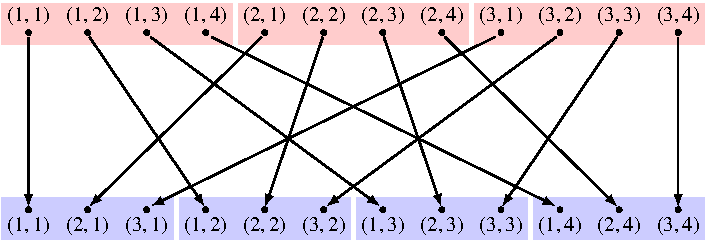
\includegraphics{chapters/060-diskret/images/permutation.pdf}
\end{center}
(hier für den Fall $n=3$ und $m=4$ dargestellt)
kann aber die gleiche Anordnung
wie in $I_m\otimes A$ erreicht werden.
Da dazu gleich viele Zeilenvertauschungen wie Spaltenvertauschungen
nötig sind, ändert sich die Determinante dadurch nicht.
Somit folgt auch
\[
\det (A\otimes I_m) = \det (I_m\otimes A) = \det(A)^m.
\qedhere
\]
\end{proof}

\begin{satz}
\label{buch:diskret:tensor:satz:det}
Für $A\in M_{n\times n}(\Bbbk)$ und $B\in M_{m\times m}(\Bbbk)$
\[
\det(A\otimes B) = \det(A)^m\det(B)^n.
\]
\end{satz}

%
% Spur 
%
\subsection{Spur von $A\otimes B$
\label{buch:diskret:tensor:subsection:spur}}
Da $A\otimes B$ aus Blöcken der Form $a_{ik}B$ besteht,
ist die Spur des Kroneckerproduktes
\begin{equation}
\operatorname{Spur}(A\otimes B)
=
\sum_{i=1}^n \operatorname{Spur}(a_{ii}B)
=
\sum_{i=1}^n a_{ii}\operatorname{Spur}(B)
=
\operatorname{Spur}(A)\operatorname{Spur}(B).
\label{buch:diskret:tensor:eqn:spur}
\end{equation}

